\documentclass[12pt, a4paper,oneside]{book}
% Подключение библиотеки
\usepackage{/Users/vladbelousov/Desktop/Semestr_4-FP-NSU/Настройка/library}

\begin{document}

\begin{titlepage}
    \thispagestyle{empty}  % Отключаем нумерацию страницы на титульном листе
    \centering
    \vspace*{1cm}  % Отступ сверху

    \textbf{\huge Конспект лекций по дисциплине}  \\[1.5cm]  % Название
    \textbf{\huge Электромагнетизм и оптика }  \\[2cm]   % Название дисциплины (оставьте пустым для добавления вручную)
    \textbf{\Large Новосибирский государственный университет} \\[0.5cm]
    \textbf{\large Физический факультет} \\[0.5cm]
    \textbf{\large 4-й семестр} \\[0.5cm]
    \textbf{\large 2025 год} \\[10cm]

    \begin{flushright}
        \large Студент: Б.В.О \\[0.5cm]  % Ваше имя
        Преподаватель: Синицкий Станислав Леонидович  % Ф.И.О. преподавателя
    \end{flushright}
\end{titlepage}

\tableofcontents  % Создание оглавления

\def\mainfile{}  % Определяем макрос для основного файла
% Условная компиляция для самостоятельной работы
\ifdefined\mainfile
    % Если это часть основного файла, не добавляем начало и конец документа
\else
    \documentclass[12pt, a4paper]{report}
    \usepackage{/Users/vladbelousov/Desktop/Semestr_4-FP-NSU/Настройка/library}
    \usepackage[utf8]{inputenc} % Подключение поддержки UTF-8
    \begin{document}
\fi

%%-------------------------------%%

\chapter{Электромагнитные волны.}

\section{Свободное электромагнитное поле. Волновое уравнение.  }

\begin{definition}[Свободное]   
означает без токов и зарядов \( \Rightarrow \rho =0 , \vec{j}= 0   \) 
\end{definition}

\[ 
\begin{aligned}
    \begin{cases}
         \displaystyle \mathrm{rot} \vec{ E} =-\frac{1}{c}\frac{\partial\vec{B}}{\partial t}, \quad \mathrm{div} \vec{B}=0 \\
        \displaystyle \mathrm{rot} \vec{H} =\frac{1}{c}\frac{\partial\vec{D}}{\partial t}, \quad \mathrm{div} \vec{D}=0     
    \end{cases} 
    + \text{Грани. условия} 
    \text{ } 
    \begin{cases}
        (B_n)| = 0 \quad (E_{\tau} )= 0 \\ 
        (D_n)| = 0 \quad (H_{\tau} )= 0 
    \end{cases}
\end{aligned}
 \] 

 \textit{Два типа векторных полей:} 

 1. Вихревые: \( \mathrm{div}\vec{F}= 0    \)  (нет источников истоков этого поля \( \Rightarrow  \) силовые линии либо замкнуты, либо уходят на бесконечность)

\begin{center}
    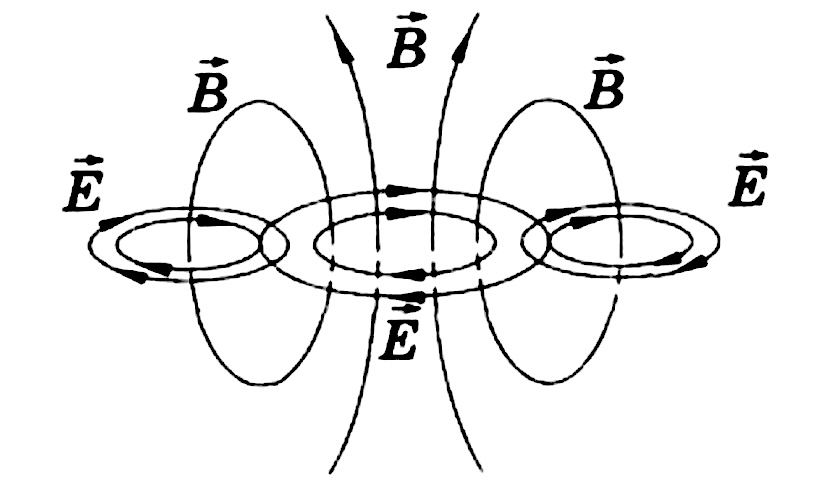
\includegraphics[width=0.3\textwidth]{/Users/vladbelousov/Desktop/Semestr_4-FP-NSU/ЭиО/Лекции_по_дням/image/1.jpeg}
\end{center}

 2. Потенциальные: \( \mathrm{rot} \vec{F} =0 \). Силовые линии выходят или входят в области стоков и истоков (где \( \mathrm{div} \vec{F} \neq 0     \)) или на бесконечности. 

\begin{center}
    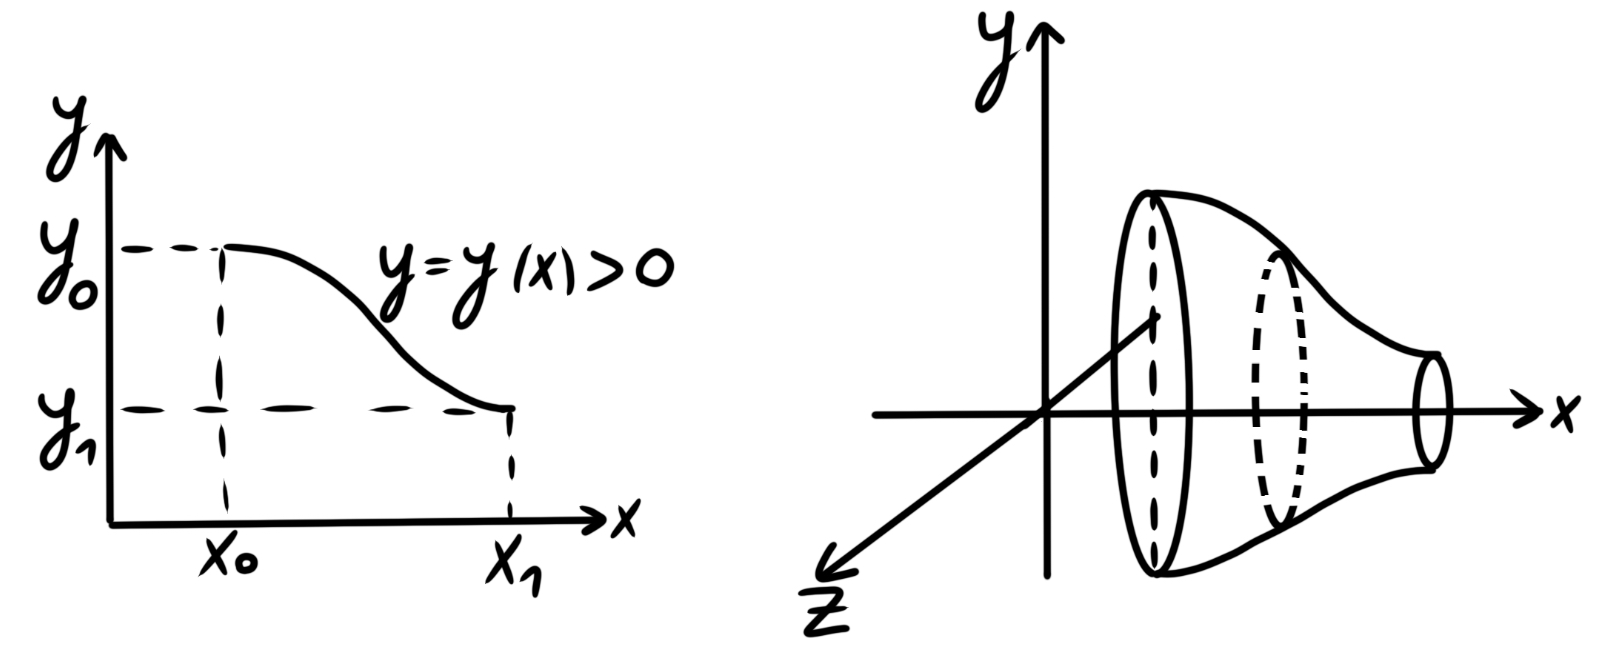
\includegraphics[width=0.5\textwidth]{/Users/vladbelousov/Desktop/Semestr_4-FP-NSU/ЭиО/Лекции_по_дням/image/2.png}
\end{center}

Далее мы будем рассматривать только вихревые поля (т.е. \( \mathrm{div} \vec{B} = 0 ,\mathrm{div} \vec{D} = 0  \))

Неизвестные 3 компоненты \( \vec{E},\vec{D},\vec{B},\vec{H}\) - 12 неизвестные функций. Мы можем решить эту систему при помощи уравнений Максвелла \( + \)  материальные уравнения: \( \vec{B}=\vec{B}(H), \vec{E}=\vec{E}(D) \).

Простая модель среды: \( \vec{B}=\mu\vec{H}, \vec{D}=\varepsilon \vec{E} \), где \( \mu = \mathrm{const}  , \varepsilon =\mathrm{const}   \), годится для вакуума (\(\mu=1, \varepsilon=1  \)) и для многих других сред/материалов при низких значения полей \( \vec{E}, \vec{B} \)  и при невысоких частотах \( f < 10^8 \) Гц. 
 
\textit{Волновое уравнение:} 

\[ 
\begin{aligned}
    \begin{cases}{}
        \displaystyle  \mathrm{rot} (\mathrm{rot} \vec{E}  )= -\frac{\mu}{c}  \frac{\partial}{\partial t} \mathrm{rot } \vec{H}= - \frac{\mu \varepsilon}{ c ^2} \frac{\partial ^2}{\partial t ^2}     \vec{E} \\
        \displaystyle \mathrm{rot} (\mathrm{rot} \vec{E}  )= \nabla \underbrace{\mathrm{div} \vec{E}}_{\frac{1}{\varepsilon} \mathrm{div}\vec{D}=0   }    - \Delta \vec{E}   
    \end{cases}
    \Rightarrow
    \begin{cases}
        \displaystyle \Delta \vec{E}- \frac{\mu \varepsilon}{c ^2} \frac{\partial ^2 \vec{E}}{\partial t ^2} =0 \\
        \displaystyle \mathrm{div}   \vec{E}=0 
    \end{cases} 
    \quad \quad  (1)
\end{aligned} 
\] 

Так же делаем с \( \mathrm{rot }(\mathrm{rot}\vec{B})\) и получаем: \( 
\begin{aligned}
    \begin{cases}
        \displaystyle  \Delta \vec{B} - \frac{\mu \varepsilon}{c ^2} \frac{\partial ^2 \vec{B}}{\partial t ^2} =0 \\
        \displaystyle \mathrm{div}   \vec{B}=0
    \end{cases}
    \quad \quad  (2)
\end{aligned} 
\)  

Согласование решений (1) и (2): 

1) Решаем (1) и \( \vec{E} \)  подстваляем в уравнение Максвелла \( \to  \vec{B} \);

2) Решаем (2) и \( \vec{B} \)  подстваляем в уравнение Максвелла \( \to  \vec{E} \);

Различные простейшие решения волнового уравнения: 

1) Плоские волны: все ненулевые компоненты полей \( \vec{ E} ,\vec{ B} \) завися от одной координаты (например от z)  и времени t; 

\begin{center}
    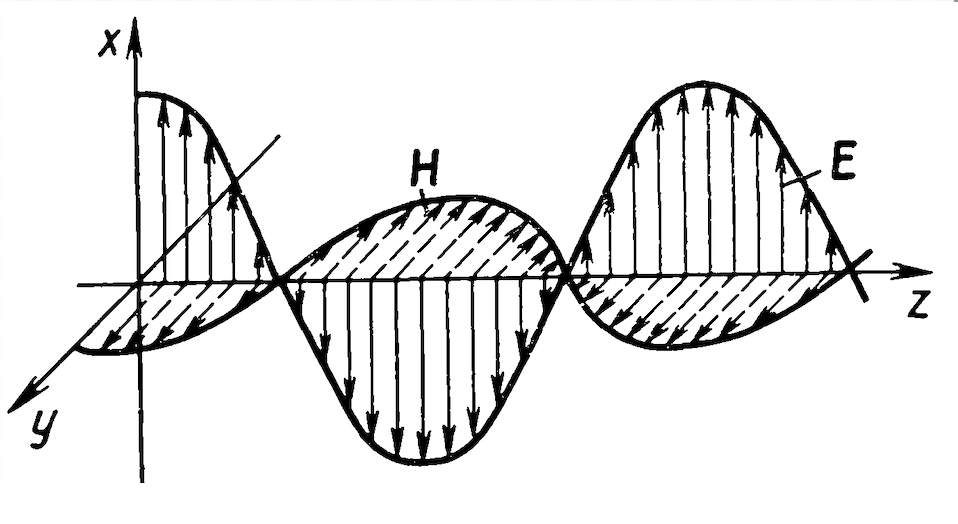
\includegraphics[width=0.3\textwidth]{/Users/vladbelousov/Desktop/Semestr_4-FP-NSU/ЭиО/Лекции_по_дням/image/3.png}
\end{center}


2) Цилиндрические волны: все ненулевые компоненты полей \( \vec{ E} ,\vec{ B} \) зависят от \( \vec{ r}  \)  - расстояния от точки наблюдения до некоторой оси (центра волны) и от времени t; 

3) Сферическая волна: все ненулевые компоненты полей \( \vec{ E} ,\vec{ B} \) зависят от \( \vec{r}  \)  - расстояния от точки наблюдения до центра волны.

\begin{center}
    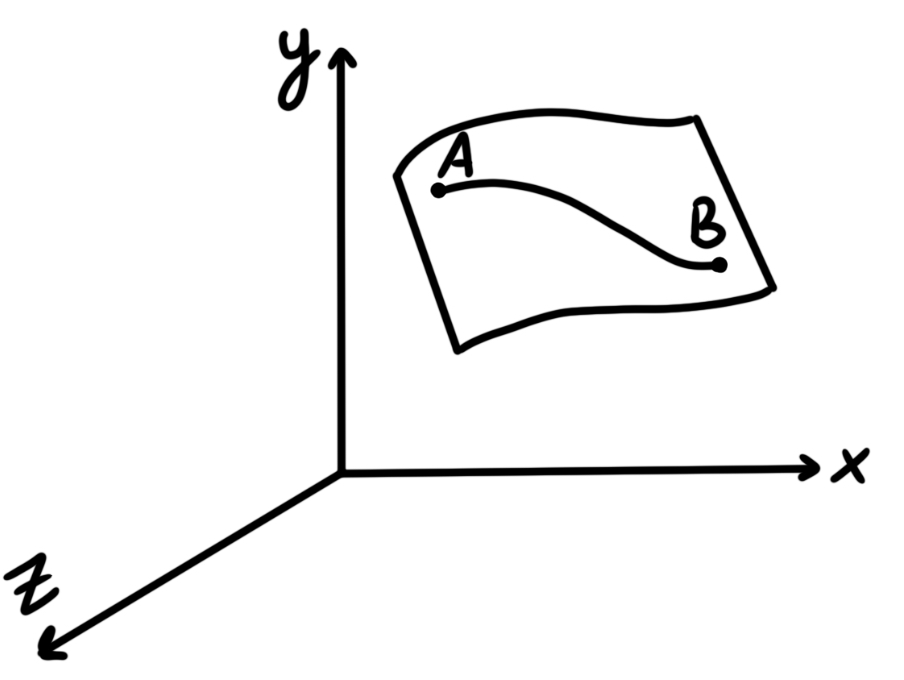
\includegraphics[width=0.3\textwidth]{/Users/vladbelousov/Desktop/Semestr_4-FP-NSU/ЭиО/Лекции_по_дням/image/4.png}
\end{center}

\section{Плоские волны. }

\[ \frac{\partial ^2 }{\partial t^2 } \vec{E} - \frac{\mu \varepsilon}{c ^2} \frac{\partial ^2 \vec{ E}}{\partial t ^2 } =0 \text{ , для примера }  E_x : \left( \frac{\partial}{\partial z} - \frac{\sqrt{\mu \varepsilon} }{c} \frac{\partial}{\partial t }   \right) \left( \frac{\partial}{\partial z} + \frac{\sqrt{\mu \varepsilon} }{c} \frac{\partial}{\partial t } \right) E_x = 0    \] 

\begin{gather*}
    \varepsilon = z - \frac{c}{ \sqrt{\mu \varepsilon} }, \quad \eta = z + \frac{c}{ \sqrt{\mu \varepsilon} } \quad ( \text{замена переменных} )  \\
    \frac{\partial}{\partial z } f ( \xi ( z,t), \eta ) = \frac{\partial f}{\partial \xi }  \underbrace{\frac{\partial \xi }{\partial z }}_{=1} + \frac{\partial f }{\partial \eta  }   \underbrace{\frac{\partial \eta }{\partial z }}_{=0}= \frac{\partial f}{\partial \xi } + \frac{\partial f}{ \partial \eta } \\
\end{gather*}

\begin{gather*}
    \frac{\sqrt{\mu \varepsilon}}{c}  \frac{\partial f }{\partial t}      = \frac{\sqrt{\mu \varepsilon}}{c} \left( \frac{\partial f }{\partial \xi } \left( - \frac{c}{\sqrt{\mu \varepsilon}}\right) + \frac{\partial f}{\partial \eta } \left( \frac{c}{\sqrt{\mu \varepsilon}}  \right)  \right)=- \frac{\partial f}{\partial \xi } + \frac{\partial f}{ \partial \eta }  \\ 
    \frac{\partial}{\partial z } \to  \frac{\partial}{\partial \xi } + \frac{\partial}{\partial \eta }, \quad \frac{\sqrt{\mu \varepsilon}}{c}\frac{\partial}{\partial t} \to \frac{\partial}{\partial \eta }- \frac{\partial }{\partial \xi } \\
    \to \left( \frac{\partial}{\partial \xi  } \frac{\partial}{\partial \eta } - \frac{\partial}{\partial \eta } + \frac{\partial}{\partial \xi  }     \right)\left( \frac{\partial}{\partial \xi  } \frac{\partial}{\partial \eta } +\frac{\partial}{\partial \eta } - \frac{\partial}{\partial \xi } \right) E_x ( \varepsilon,\mu)= 0 \quad 4 \frac{\partial}{ \partial\mu \partial\varepsilon}E_x ( \varepsilon,\mu)= 0  
\end{gather*} 

Решения являются произвольные функции \( f(\xi) , f(\eta) \)

\begin{gather*}
    E_x (z,t) = f \left(z- \frac{c}{\sqrt{ \mu \varepsilon }}   \right)+ g \left(  z+ \frac{c}{\sqrt{ \mu \varepsilon }} \right) \\ 
    E_y (z,t) = p \left(z- \frac{c}{\sqrt{ \mu \varepsilon }}   \right)+ h \left(  z+ \frac{c}{\sqrt{ \mu \varepsilon }} \right) \\ 
    \text{где } \forall   f,g,p,h 
\end{gather*}

Свойства плоских волн: 

1) \( E_z = 0 , B_z =0  \) 

\[ \displaystyle  \mathrm{div}\vec{D}=\varepsilon \vec{E} =0 = \varepsilon \left( \frac{\partial E_x }{\partial x }+ \frac{\partial E_y }{\partial y }+\frac{\partial E_z }{\partial z }  \right) \text{первые два члена равны нулю.}    \]


\( \Rightarrow  E_z\) - не зависит от z \( \Rightarrow  \) не зависит от t - этот случай не соответствует волновому полю. 

Пример: 

\begin{center}
    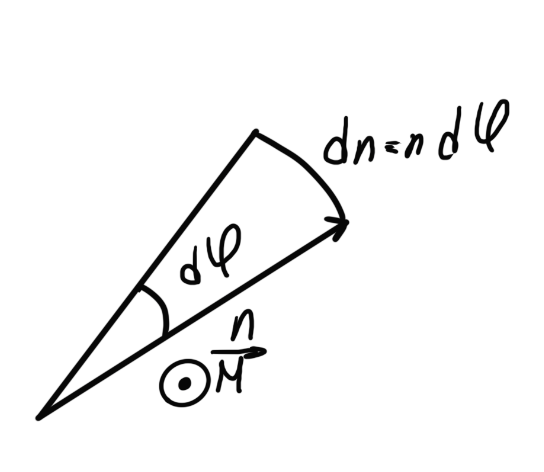
\includegraphics[width=0.7\textwidth]{/Users/vladbelousov/Desktop/Semestr_4-FP-NSU/ЭиО/Лекции_по_дням/image/5.png}
\end{center}

В максимуме \( z - \frac{c}{ \sqrt{ \mu \varepsilon}} = 0   \) 

\[ \displaystyle  \underbrace{\frac{dz}{dt} }_{V_{\Phi }  }- \frac{c}{\sqrt{ \mu \varepsilon}}=0   \] 

2) Связь поперечных полей в плоской волне: 

\( \displaystyle  \sqrt{\varepsilon} \vec{E} = \sqrt{ \mu} [\vec{H}\times \vec{n}], \quad \sqrt{\mu} \vec{H} = \sqrt{ \varepsilon} [\vec{n}\times \vec{E}] \)

где \( \vec{n } \) - единичный вектор направления движения волны(\(  \vec{E} \perp \vec{B} \perp \vec{n} \)). 

3) \( \displaystyle \varepsilon E ^2 = \mu [ \displaystyle \vec{H}\times  \vec{n }] ^2 = \mu H ^2 n ^2 = \mu H ^2 | : 8 \pi \Rightarrow W_E = \frac{\varepsilon E ^2 }{8 \pi} =\frac{\mu B ^2 }{8 \pi} = W_B  \) 

4) \( \vec{S}= \frac{c}{4 \pi}   [ \vec{E}\times \vec{H }] \) - плотность потока энергии. 

\begin{gather*}
    \vec{S} = \frac{c}{4 \pi} [\vec{E } \times  \sqrt{\frac{\varepsilon}{\mu} }[\vec{n }\times  \vec{E}]]= \frac{c \varepsilon}{4 \pi \sqrt{ \mu \varepsilon}} \left( \vec{n}( \vec{E}\vec{E}) - \underbrace{\vec{E}( \vec{n }\vec{E})}_{=0}   \right)= \frac{c}{\sqrt{ \mu \varepsilon}} \vec{n} \left( \underbrace{\frac{\varepsilon E ^2 }{8 \pi}}_{W_E}  +\underbrace{\frac{\mu B ^2 }{8 \pi}  }_{W_B}  \right)   
\end{gather*}

\section{Плоские монохроматические волные (ПМВ).}

\( E_x, E_e, B_x, B_y \sim e^{-i \omega t}   \) 

\text{ }

\begin{minipage}{0.5\textwidth}
    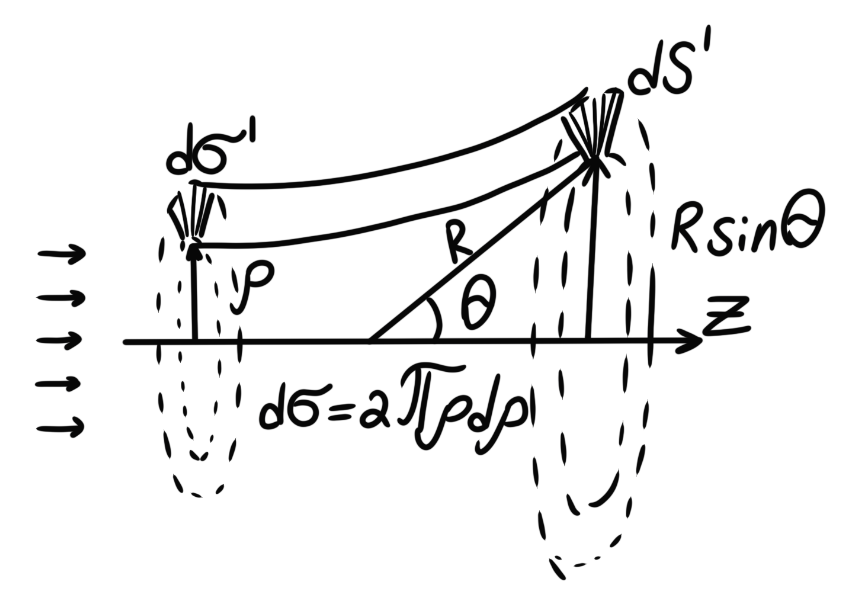
\includegraphics[width=0.8\textwidth]{/Users/vladbelousov/Desktop/Semestr_4-FP-NSU/ЭиО/Лекции_по_дням/image/6.png}
\end{minipage}
\begin{minipage}{0.5\textwidth}
    \text{В плоскости } \( z = z_0 , \vec{E}( z_0,t )= \vec{E_0}e^{-i \omega t} \) 
\end{minipage}

\begin{gather*}
  \displaystyle   \vec{E}( z,t)= \vec{E_0} e^{\frac{i \omega \sqrt{ \mu \varepsilon}}{c} \left( z- \frac{c}{\sqrt{\mu \varepsilon}} t -z_0  \right) } \underbrace{\vec{E_0}e^{-\frac{i \omega \sqrt{ \mu \varepsilon}}{c}z_0} }_{\vec{E_{00}}} \cdot \underbrace{e^{\frac{i \omega \sqrt{ \mu \varepsilon}}{c} \left( z - \frac{c}{\sqrt{ \mu \varepsilon}}t  \right)} } _{f (z - \frac{c}{\sqrt{ \mu \varepsilon}}t)}   
\end{gather*}

\( \vec{E_0 } \perp \vec{n} = \vec{e_z} \Rightarrow \vec{E_0}=c_1 \vec{e_x}+ c_2 \vec{e_y}, c_1 \text{ и } c_2   \) - произвольные комплексные числа. 

\begin{definition}
    Волновое число \( k = \frac{\omega \sqrt{ \mu \varepsilon}}{c} = \frac{\omega}{V_{\text{волн.} } }   \) 
\end{definition}

\[ \displaystyle \vec{E}= \vec{E_{00}}e^{ikz- i \omega t } - \text{ для волны с } \vec{n} = \vec{e_z}, \qquad \vec{E}= \vec{E_{000}}e^{-ikz- i \omega t } - \text{ для волны с } \vec{n} = \vec{-e_z}  \] 

Универсальная запись полей ПМВ: 

\begin{center}
    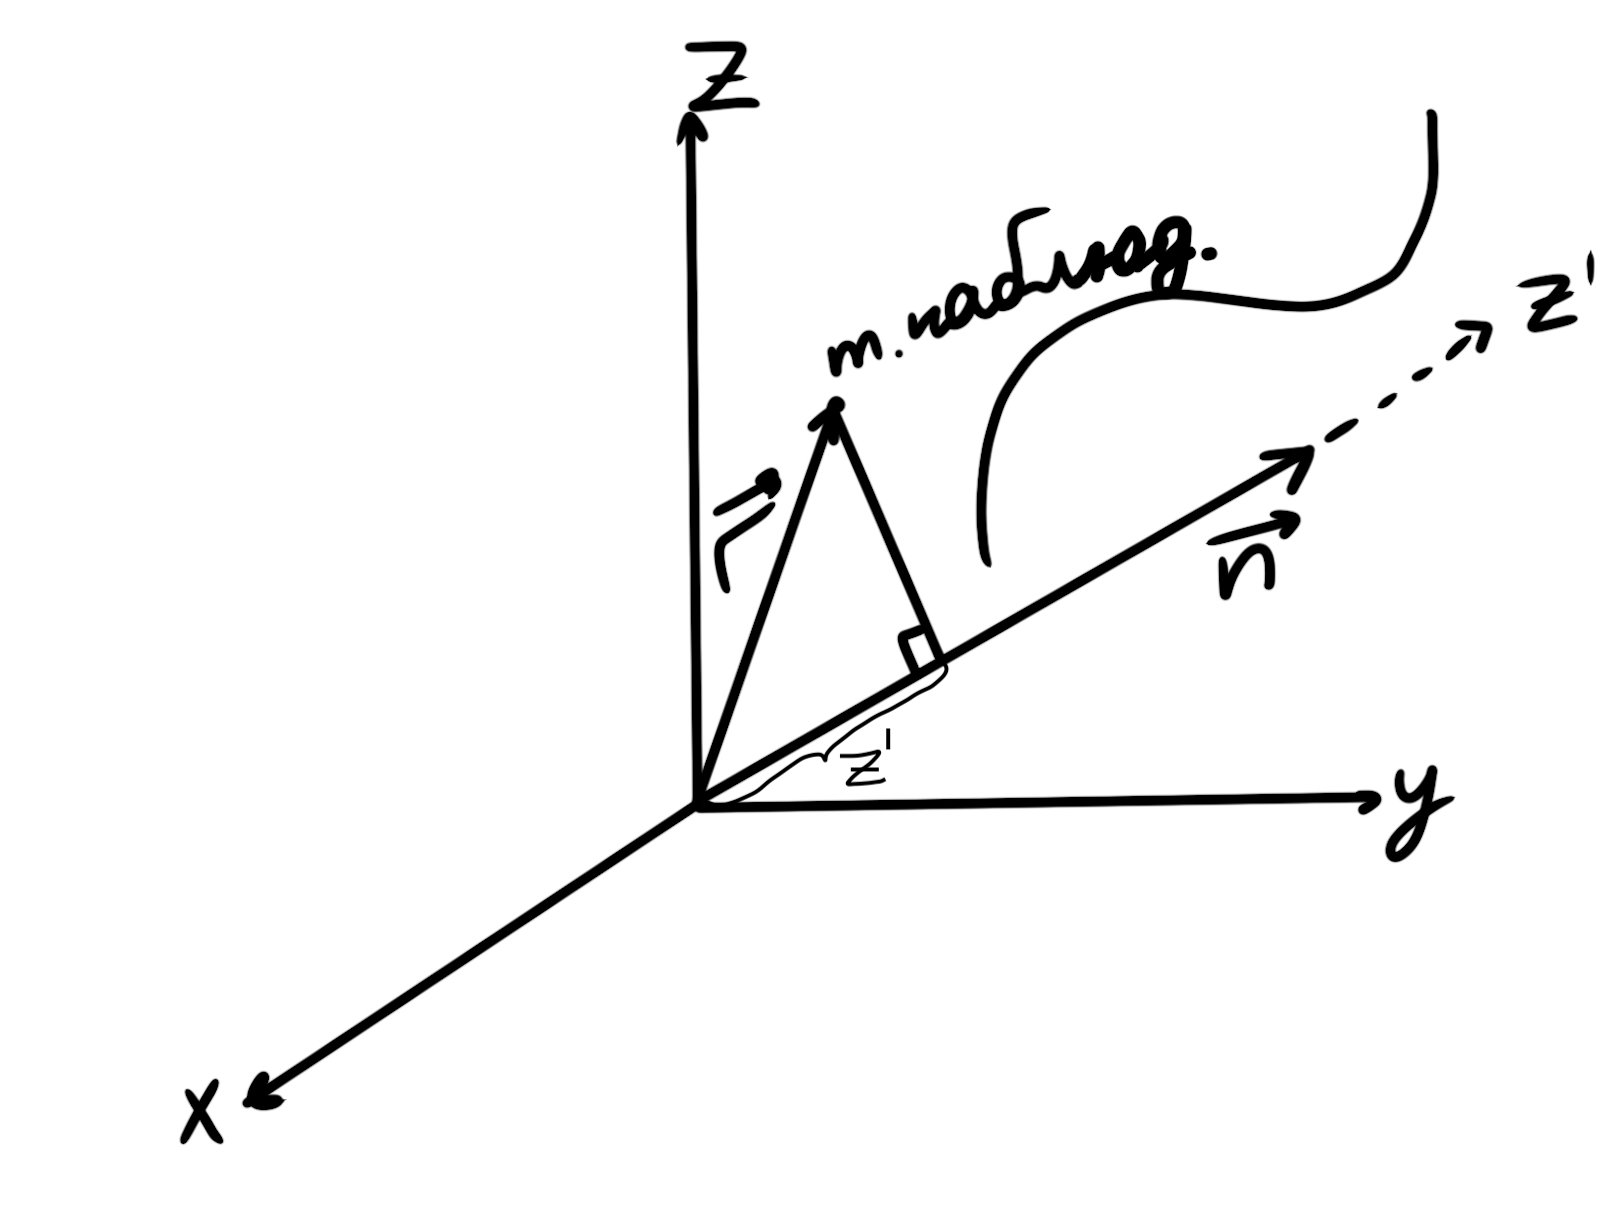
\includegraphics[width=0.4\textwidth]{/Users/vladbelousov/Desktop/Semestr_4-FP-NSU/ЭиО/Лекции_по_дням/image/7.png}
\end{center}

\[ \begin{aligned}
    \begin{cases}
        \vec{E}( z', t)= \vec{E_0 }e^{ikz' - i \omega t } \\  
        z'= (\vec{n}, \vec{r})
    \end{cases}
    \Rightarrow
    \vec{E}( z', t)= \vec{E_0}e^{ik(\vec{n}, \vec{r}) - i \omega t }= \vec{E_0}e^{ik(\vec{k}, \vec{r}) - i \omega t }
\end{aligned} \] 
%%-------------------------------%%

% Закрытие документа, если файл компилируется отдельно
\ifdefined\mainfile
    % Если это основной файл, не нужно заканчивать документ
\else
    \end{document}
\fi

\end{document}
